\documentclass[12pt]{article} 
%\geometry{verbose,letterpaper,tmargin=2.54cm,bmargin=2.54cm,lmargin=2.54cm,rmargin=2.54cm} 
\usepackage{setspace}%
\usepackage{lineno}%
\usepackage{authblk}%
\usepackage[parfill]{parskip}
\usepackage{hyperref}
\usepackage{graphicx}
\usepackage{float}
\usepackage{rotating}
\usepackage{mathtools}%
\usepackage[backend=biber,style= ele,natbib=true]{biblatex}
\addbibresource{Stable_Isotopes_and_Fatty_acids.bib} 

\makeatletter%
\def\@maketitle{%
  \vskip 2em%
  \begin{center}%
%  \let \footnote \thanks
    {\Large\bfseries \@title \par}%
    \vskip 1.5em%
    {\normalsize
      \lineskip .5em%
      \begin{tabular}[t]{c}%
        \@author
      \end{tabular}\par}%
    \vskip 1em%
    {\normalsize \@date}%
  \end{center}%
  \par
  \vskip 1.5em}
\makeatother

\begin{document}


\title{Overall model performance and determinants of estimation accuracy}

\renewcommand\footnotemark{}

\author{Philipp Neubauer*}\thanks{*Corresponding author electronic address: neubauer.phil@gmail.com}%
\affil{Dragonfly Science,\\PO Box 27535, Wellington 6141, New Zealand}%

\author{Olaf P. Jensen}%
\affil{Institute of Marine and Coastal Sciences\\Rutgers University, New Brunswick, NJ 08901, USA}%

\maketitle

\section{Simulations to determine factors influencing model performance} 

\subsection{Overall determinants of model performance}

Performance of our model can be assessed by measuring the accuracy of estimated
diet proportions, which can be tested using simulations. There are a
number of potential determinants of accuracy, such as (i) the data used to infer diet
proportions, (ii) the
model setup as well as (iii) the choice of posterior summary as point
estimate of true diet proportions.

At the level of the data input (i), the resolution that the FAPs
provide for a given set of potential prey species (i.e., separation of
distributions in FAP space), as well as their
co-linearity in FAP space will be major determinants of
accuracy. Furthermore, the accuracy of conversion coefficients will
bear strongly on the model's ability to
estimate correct diet proportions
\citep{iverson_quantitative_2004}. In the following, we will
illustrate the respective effect of each of these factors using simulations.

For the model setup (ii), the model formulation itself (i.e., major assumptions) may more or
less suited for the data at hand, leading
to variability in accuracy, or specific components of the model may be
more or less suited for a particular dataset. The latter case refers
to distributional forms of priors and likelihoods formulated
in the model, and can be assessed by varying priors and distributional
assumptions, whereas the former (e.g., model-mis-specification) is more
difficult to measure and should be carefully assessed by the
practitioner both \emph{a priori} and by checking the model output.
 
To illustrate model performance relative to characteristics of the
input data (i), we performed a series of 675 standardized simulations that
were designed to isolate the relative effect of the evenness of diet proportions,
the separation of prey distributions in FAP space, as well as their
co-linearity in that space. We further performed simulations to assess
the effects of conversion coefficients on diet proportion
estimates. As the model setup (ii) and appropriateness of posterior
summaries (iii) will depend on both the input data and actual (here,
simulated) diet proportions, we standardized the model setup (and
priors). For each simulation, we drew 20 samples, containing 12
FAs from each of 4 prey species
at random from a Dirichlet distribution with randomly chosen
parameters. We then calculated expected predator signatures for 3
predators according to random diet proportions drawn from a random
population mean. We then used a model with default priors to estimate
population level diet proportions for these predators. 

To assess the accuracy in estimated diet proportions, we used posterior means as point estimates of inferred diet
proportions for all simulations. We then used a log-linear model to
quantify the influence of diet evenness, co-linearity and source separation in FAP
space, as well as their interaction, on differences between simulated
and inferred diet proportions as measured by the Aitchison distance \citep{aitchison_logratio_2000}. We used stepwise model selection using
AIC implemented in R (the step function) to select
influential determinants of accuracy as well as their interactions.

\subsection{Conversion coefficients and their importance for diet
  estimates}

Fatty acids are not always assimilated in direct proportion to their
prevalence in a consumer’s diet. Controlled feeding studies suggest
that the relative rate at which individual fatty acids are assimilated
may vary by predator, prey, and fatty acid \citep{rosen_effects_2012}. While a detailed discussion of the biochemistry of fatty acid
assimilation is beyond the scope of this paper, it is important to
note that these coefficients are difficult to obtain from anything but
controlled feeding experiments, which in turn are difficult to realize
on animals that are not easily cultured or kept in captivity. Many
studies that have used FAP to estimate diets have noted potential
biases from unknown conversion coefficients \citep[e.g.][]{iverson_quantitative_2004,meynier_quantitative_2010}, and results from
experimental studies confirm that the assumption of no and/or false
conversion coefficients can bias diet estimates \citep{rosen_effects_2012}. Furthermore,
  even closely related species may have significantly different
  conversion coefficients for different fatty acids and prey items
  \citep{rosen_effects_2012}, and it may therefore be difficult to use a
  set of coefficients from a closely related predator or prey species
  for any diet study.

We assessed the effect of ignoring conversion coefficients in our
model by estimating simulated diet proportions, first setting
$\kappa_s$ to the true means and variances used to simulate the data,
and then running the model with $\kappa_s = 1$, with a prior variance set to the
variance $\kappa$. To estimate the diet proportions, we used our model on
simulated FAPs composed of 12 FAs, simulating prey and FA specific
conversion coefficients from a normal distribution centered on 1 and
truncated at 0,
with increasing variance. This was repeated for the 100 simulated datasets for
each of six increments (from 0 to 0.5) in the variance of simulated
$\kappa$. 

\section{Simulation results}

Simulations illustrated that inferred diets using posterior means were sensitive to
separation of diet distributions ($P<0.05$) and diet
evenness ($P<0.001$), with more even and well separated diets leading to
more accurate diet estimates. Co-linearity was not significant in the
linear model, likely due to the simulation setup of only including 4
sources. \citet{blanchard_inference_2011} found a strong influence of
source co-linearity with a higher number of sources, and the same
should be expected here as a mathematical inevitability. 

The interaction between source separation and diet evenness, demonstrated that uneven diets only
consistently affect model inferences when sources are not well
separated: with increasing separation (\autoref{fig:test_error}), the uncertainty about the
influence of diet evenness on estimation accuracy increases
substantially.

\begin{sidewaysfigure}
  \centering   
      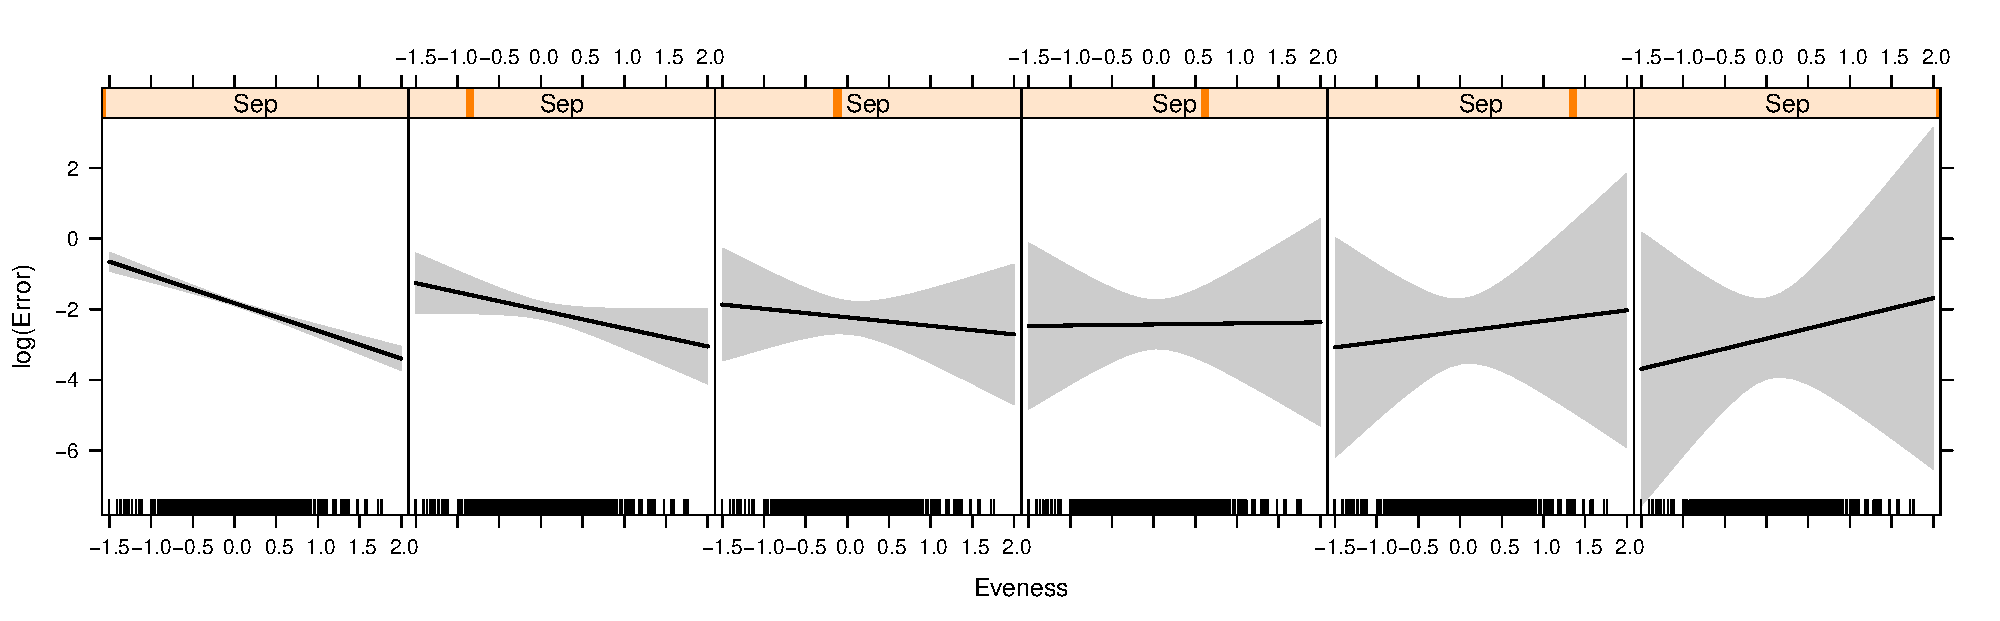
\includegraphics[width=1\textwidth]{figures/test_error.pdf}  
       \caption{Interactive effect of source separation (Sep) and diet
       evenness on log distances between simulated diet
         proportions and posterior means of diet proportions.}
\label{fig:test_error}
\end{sidewaysfigure}

With adequate resolution and known conversion coefficients, diet
estimates are usually precise (\autoref{fig:cc_test}). When conversion
coefficients are unknown and set to 1, we found that, on average, the
distances between (transformed) diet proportion vectors and their
estimates increased with the variance of the conversion coefficients
$\kappa$. There is no noticeable difference between specifying normal
or log-normal models for conversion coefficients. This contrasts with
models with specified $\kappa$, which have consistently high accuracy, mainly associated with taking point estimates from the posterior distribution to calculate the distance.


\begin{figure}[H]
  \begin{center}    
      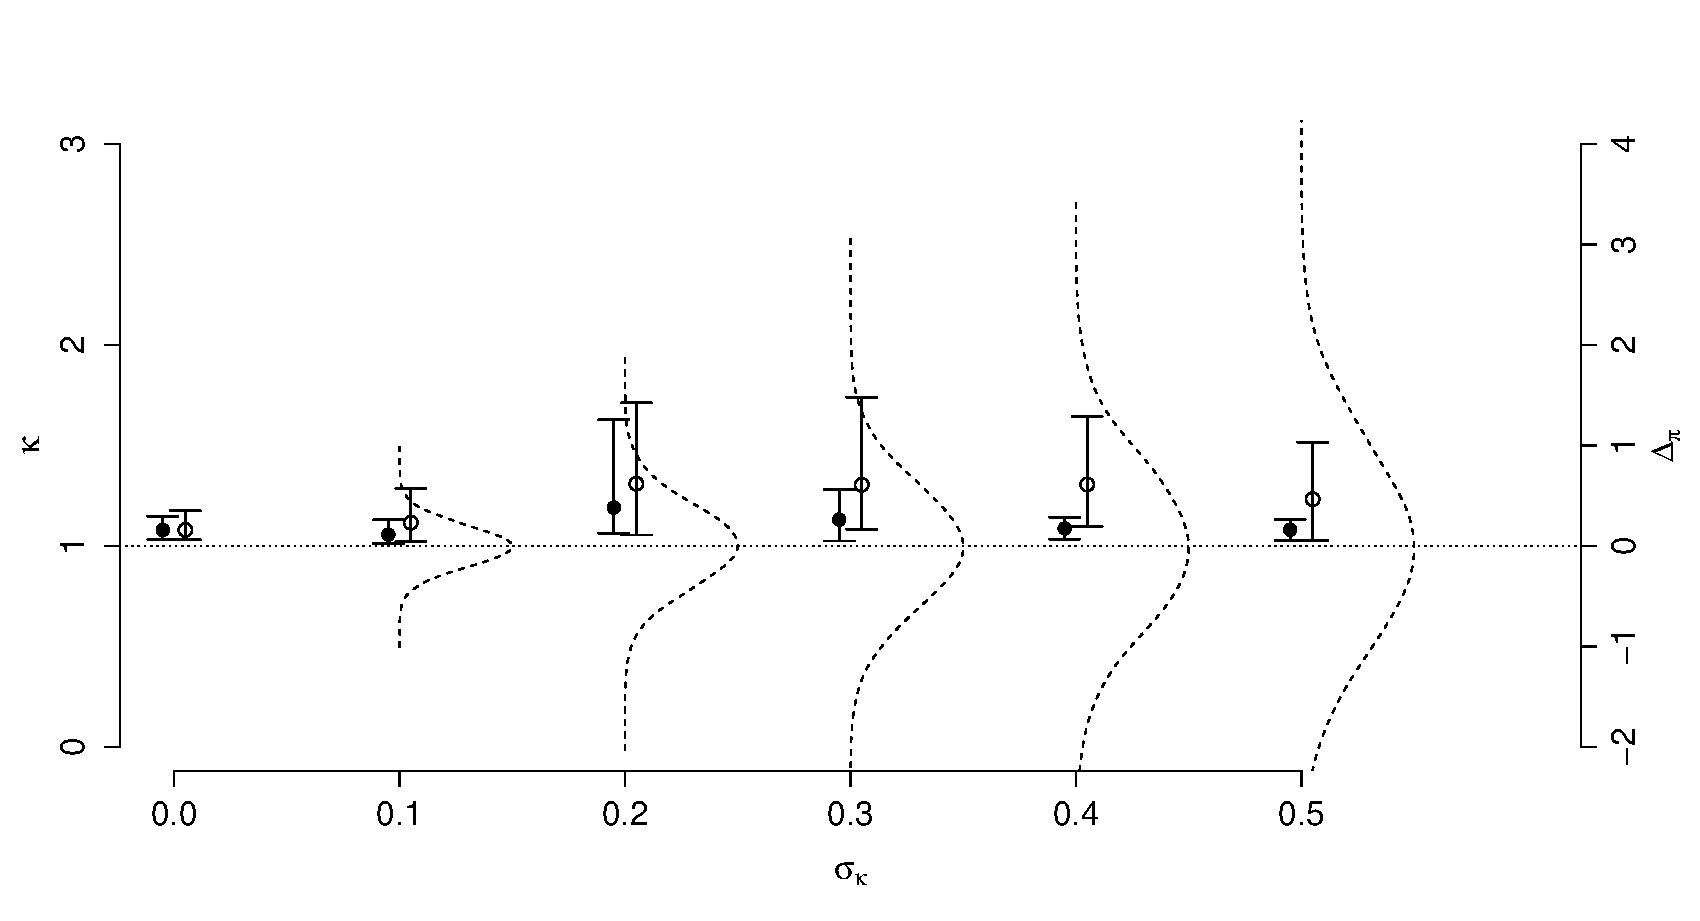
\includegraphics[width=1\textwidth]{figures/CC_error.pdf}  
       \caption{Estimated distance $\Delta_\pi$ between simulated diet
         proportions and point estimates of diet proportions, as a function on variance of
         conversion coefficients ($\sigma_\kappa$). Circles are mean distances from point
         estimates for diet contributions from 100
         simulations, error bars are sd of distances. Filled circles show distances from estimates with correct conversion coefficients, open symbols illustrate distances when ignoring these coefficients and instead setting a large variance to reflect uncertainty.}
\label{fig:cc_test}
\end{center}
\end{figure}


Note that much of the increase in the distance $\Delta_\pi$ between simulated diet
         proportions and point estimates of diet proportions when
ignoring conversion coefficients also results from making point
estimates of diet proportions from skewed and wide distributions,
reflecting slow or non-convergence of MCMC and/or uncertainty in diet
estimates (\autoref{fig:bad_cc_plot}).

\begin{figure}[H]
  \begin{center}    
      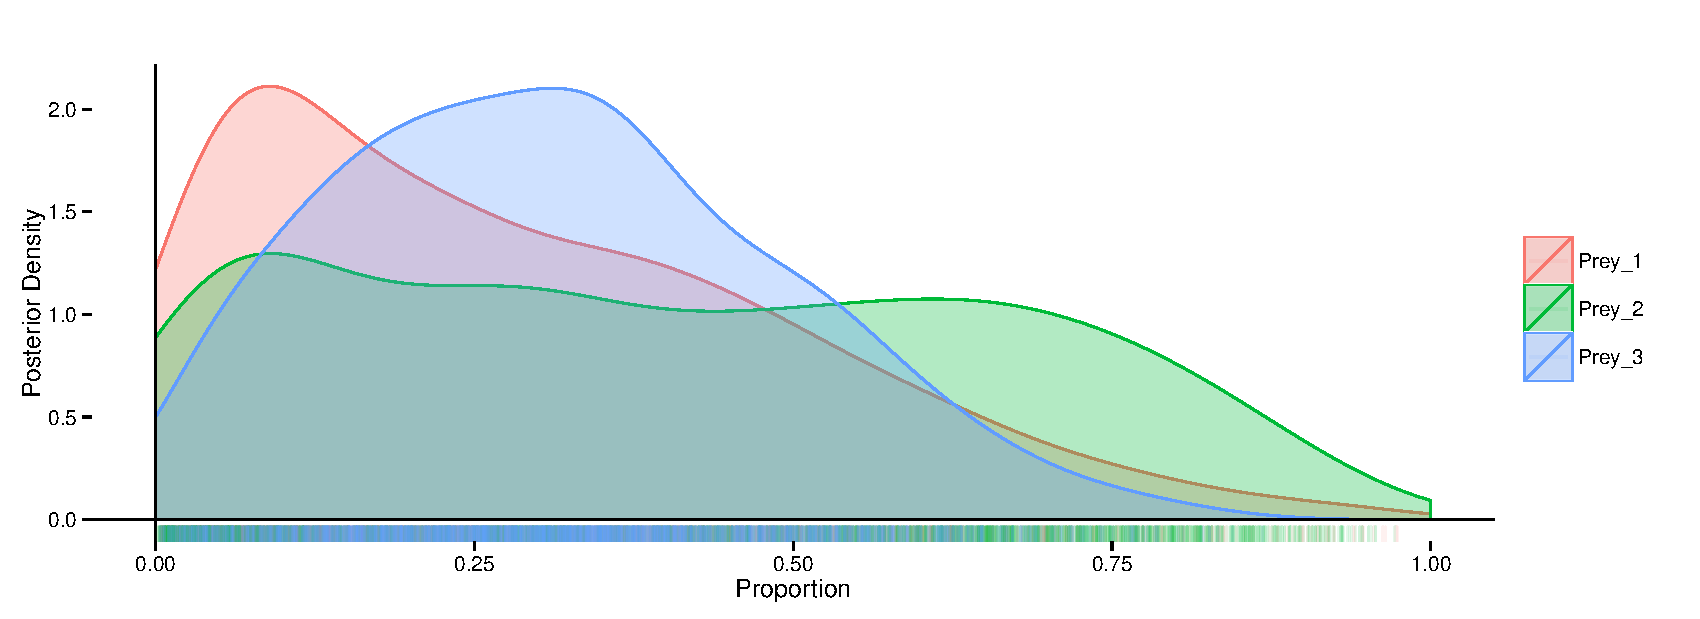
\includegraphics[width=1\textwidth]{figures/bad_cc_plot.pdf}  
       \caption{Example of posterior distributions for a simulation
         with $kappa$ set to one, showing the difficulty to obtain
         reasonable point estimates with ignored conversion
         coefficients in this case.}
\label{fig:bad_cc_plot}
\end{center}
\end{figure}



\printbibliography

\end{document}